%\documentclass[10pt]{llncs}


%\usepackage{amsmath}
%\usepackage{graphicx}
%\usepackage{subfigure}

%\usepackage{alltt}
%\usepackage{placeins}

%\usepackage{fancyvrb}


   \DefineVerbatimEnvironment
     {code}{Verbatim}
     {fontsize=\small,xleftmargin=0.6cm,samepage=true}

%\begin{document}


%\title{Obsidian:\\A Domain Specific Embedded Language\\for Parallel Programming of Graphics Processors}
       

%\author{Joel Svensson \and Mary Sheeran \and Koen Claessen}
%\institute{Chalmers University of Technology, G\"oteborg, Sweden}

%\date{}
%\maketitle

\subsection*{Abstract}

We present a domain specific language, embedded in Haskell, for general
purpose parallel programming on GPUs. Our intention is to explore the use of
{\em connection patterns} in parallel programming. We briefly present our
earlier work on hardware generation, and outline the current state of GPU
architectures and programming models. Finally, we present the current status
of the {\em Obsidian} project, which aims to make GPU programming easier,
without relinquishing detailed control of GPU resources. Both a programming
example and some details of the implementation are presented. This is a
report on work in progress.

%\end{abstract}
\subsection{Introduction} 

Sorting is an ever important, ever fascinating field of computer
science. The introduction of GPUs has introduced new challenges in
designing fast sorting algorithms.

This paper focuses on counting sort together with a variation which
removes duplicate elements. We call this variation
{\em occurrence sort}. Counting sort is a non-comparing sort
suitable for parallel implementation. The occurrence sort variation 
presented here is interesting because it seems to be a particularly
good fit for executing on the GPU. It has a very natural functional,
data-parallel implementation. We believe we are the first to study
this variation in the literature.

These algorithms are explored in Obsidian \cite{JSLIC,PUSH}, a domain
specific language targeting GPU programming. The goal of Obsidian is
to strike a balance between high-level constructs and low-level control. 
We want to provide the programmer with a set of tools for low-level 
experimentation with the details that influence performance when 
implementing GPU kernels. The counting sort
case study shows that Obsidian generates competitive kernels with
relatively little programmer effort. That Obsidian is an embedded language 
allows us to rapidly experiment with the addition of features and with varying 
programming idioms. The version used in this case study
adds global arrays and atomic instructions to Obsidian, see section 
\ref{sec:OBSHist}. 

The contributions of this paper are:
\begin{itemize}
\item We provide measurements (section \ref{sec:CSORTBenchmarks}) showing
  that counting sort is a competitive algorithm for sorting keys on the GPU,
  outperforming the sorting implementation in the library
  Thrust\cite{THRUST} in many cases.
\item Occurrence sort is shown to be particularly
  suitable for implementing on the GPU (section \ref{sec:occur}) and
  performs well (section \ref{sec:CSORTBenchmarks}).
\item The Obsidian implementation of the two sorting algorithms is
  detailed along with the generated CUDA (sections
  \ref{sec:Obsidian} and \ref{sec:parallel}).
\end{itemize}


\subsubsection{Related work} 

Sorting has applications in the computer graphics field \cite{sintorn}. 
Example instances of sorting and duplicate element removal in computer graphics 
can be identified in references \cite{Olsson} and \cite{Karras}. Another example 
of where sorting and the removal of duplicates have applications is 
in databases \cite{REMOVEDUPS}. 

%% Sorting on the GPU is interesting both for computer graphics
%% applications \cite{SINTORN} and for using the GPU to offload the
%% processor, for example in database applications \cite{REMOVEDUPS}.

The paper \cite{CSORT} implements counting sort in CUDA, and also optimisations 
that overlap computations with transferring data to and from the GPU.
Our work differs by being implemented in a high-level embedded
language and also by implementation of the occurrence sort variant of counting sort. We have not been concerned with
trying to overlap computations and data transfer, but have instead
focused solely on computations within the GPU.

Obsidian is a high-level embedded language for GPU
programming. Other such approaches include Accelerate
\cite{Acc} and Nikola \cite{NIKOLA}. Accelerate and Nikola both take an even
higher level approach compared to Obsidian and abstract more from GPU
details. Another example of providing a high-level interface to
programming the GPU is the C++ library Thrust \cite{THRUST}.
%\cite{FELDSPAR} 

%% With the Obsidian language we raise the level of abstraction for 
%% GPU kernel implementation. In order to generate CUDA code that performs well, 
%% Obsidian tries to strike a balance between high level constructs and low level 
%% control. 

%% This paper describes a case study. We implement a sorting algorithm known 
%% as counting sort. As an extra bonus we explore a variant of counting sort 
%% that can be given a nice purely functional description and lends itself well 
%% to parallelisation. The experimental results in section \ref{sec:Benchmarks} 
%% compares the performance of the counting sort algorithm we implement here to 
%% the NVIDIA Thrust \cite{THRUST} library. The Obsidian generated kernels perform
%% very well at relatively light work effort. 

%% Counting sort places new demands on Obsidian and points out areas of 
%% improvement. Some left to do, some already implemented and used here. 
%% First, in order to implement counting sort we added atomic operations to 
%% Obsidian. However, currently you can only use them by very low level features 
%% of Obsidian. This is shown in section \ref{sec:parallel}. This paper also 
%% shows for the first time the new global arrays and what they can be used for.
   

%Vague intro ideas.
%\begin{itemize}
%  \item Quickly, what is our idea. 
%  \item Why is this sorting useful.
%        (Or is i just a fun experiment.) 
%  \item GPUs are pretty cool 
%  \item This is an Obsidian case-study. 
%  \item Sneak in ref to Feldspar.
%  
%\end{itemize} 

%\cite{CSORT} 
%\cite{FELDSPAR}

\subsection{Connection patterns for hardware design and parallel programming}\label{sec:combinators}

Connection patterns that capture common ways to connect sub-circuits into larger structures have been central to our research on functional and relational languages for hardware design.
Inspired by Backus' FP language, Sheeran's early work on $\mu$FP made use of
{\em combining forms} with geometric interpretations~\cite{SheeranLFP84}. This approach
to capturing circuit regularity was also influenced by contact
with designers of regular array circuits in industry -- see reference~\cite{SheeranJUCS} for an overview of this and much other work on functional programming and hardware design.

Later work on (our) Ruby considered the use of binary relations, rather than functions in specifying hardware~\cite{LyngbyRuby}. Lava builds upon these ideas, but also gains much in expressiveness and flexibility by being embedded in Haskell~\cite{lavaICFP,ClaessenThesis}.
The user writes what look like circuit descriptions, but are in fact circuit {\em generators}. Commonly used {\em connection patterns} are captured by higher order functions.

For example, an important pattern is parallel prefix or scan. Given inputs\newline $[x_0, x_1 \ldots x_{n-1}]$, the prefix problem is to compute each $x_0 \circ x_1 \circ \ldots \circ x_j$ for $0 \leq j < n$, for $\circ$ an associative, but not necessarily commutative, operator. For example, the prefix sum of {\tt [1..10]} is {\tt [1,3,6,10,15,21,28,36,45,55]}. There is an obvious sequential solution, but in circuit design one is often aiming for a circuit that exploits parallelism, and so is faster (but also larger). In a construction attributed to Sklansky, one can perform the prefix
calculation by first, recursively, performing the prefix calculation on 
each half of the input, and then combining (via the operator) the last output of the first of these
recursive calls with each of the outputs of the second.
For instance, to calculate the prefix sum of {\tt [1..10]}, one can compute the prefix
sums of {\tt [1..5]} and {\tt [6..10]}, giving {\tt [1,3,6,10,15]}
and {\tt [6,13,21,30,40]}, respectively. 
The final step is to add the last element of the output of the first recursive call ({\tt 15}) to each element of
the output of the second.

To express the construction in Lava, we make use of two connection patterns.\newline
{\tt two :: ([a] -> [b]) -> [a] -> [b]} applies its component to
the top and bottom halves of the input list, concatenating the two sub-lists
that result from these applications.
Thus, {\tt two (sklansky plus)} applied to {\tt [1..10]} gives {\tt [1,3,6,} {\tt10,15,6,13,21,30,40]}.
Left-to-right serial composition has type
{\tt (a -> b) -> (b -> c) -> a -> c} and is written as infix {\tt ->-}.
The description of the construction mixes the use of connection patterns, giving a form of reuse, with the naming of ``wires''.

\begin{code}
sklansky :: ((t, t) -> t) -> [t] -> [t]
sklansky op [a] = [a]
sklansky op as = (two (sklansky op) ->- sfan) as
  where
    sfan as = a1s ++ a2s'
      where
        (a1s,a2s) = splitAt ((length as + 1) `div` 2) as
        a2s'      = [op(last a1s,a) | a <- a2s]

*Main> simulate (sklansky plus) [1..10]
[1,3,6,10,15,21,28,36,45,55]
\end{code}

Lava supports simulation, formal verification and netlist generation from definitions like this. Circuit descriptions are {\em run} (in fact symbolically evaluated) in order to produce an intermediate representation, which is in turn written out in various formats (for fixed size instances). So this is an example of {\em staged programming}~\cite{Taha03}.

The Sklansky construction is one way to implement parallel prefix, and there are many others, see for instance Hinze's excellent survey~\cite{Hinze}.
Those who develop prefix algorithms suitable for hardware implementation use a standard notation to represent
the resulting networks. Data flows from top to bottom and
the least significant input is at top left. Black dots represent
operators.
For example, Figure~\ref{fig:skl32} shows the
recursive Sklansky construction for 32 inputs. 
%
\begin{figure}%
\begin{center}
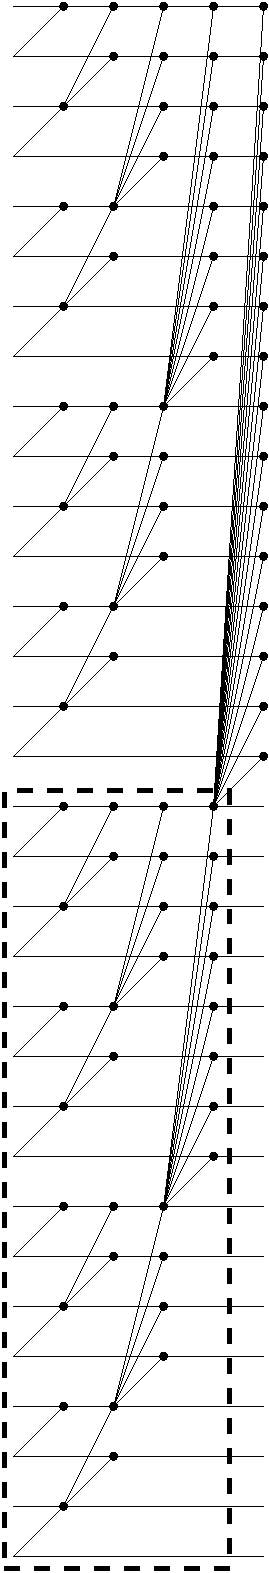
\includegraphics[bb=0 0 123 748, angle=270, scale=0.4]{./ifl/skl32.pdf}
\caption{The Sklansky construction for $32$ inputs. 
It recursively computes the parallel prefix for each half of the inputs (corresponding to the use of {\tt two} in the definition) and then combines the last output of the lower (left) half with each of the outputs of the upper (right) half. The dotted box outlines the recursive call on the lower half of the inputs.}\label{fig:skl32}
\end{center}
\end{figure}

In this work, we plan to investigate the use of connection patterns, and more generally an emphasis on {\em structure}, in parallel programming.
We have chosen to target GPUs partly because of available expertise among our colleagues at Chalmers, and partly because reading papers about General Purpose GPU (GPGPU) programming gave us a sense of d{\'e}j\`a vu. Programs are illustrated graphically, and bear a remarkable resemblance to circuit modules that we have
generated in the past using Lava. We see an opportunity here, as there is an extensive literature, going back to the 1960s, about implementing algorithms on silicon that may provide clues
about implementing algorithms on GPUs. This literature does not seem to have yet been scrutinised by the Data Parallel Programming or GPGPU communities.
This is possibly because GPUs are moving closer to simply being data parallel machines, and so work on library functions has taken inspiration from earlier work on Data Parallel Programming, such as Blelloch's NESL~\cite{NESL}. But some of the restrictions from the early data parallel machines no longer hold today; for instance broadcasting a value to many processors was expensive in the past, but is much easier to do on modern GPUs. So a construction like Sklansky, which requires such broadcasting, should now be reconsidered, and indeed we have found it to give good results in our initial experiments (writing directly in CUDA). In general, it makes sense to spread the net beyond the standard data parallel programming literature when looking for inspiration in parallel algorithm design. We plan to explore the use of ``old'' circuit design ideas in programming library functions for GPUs.

Below, we briefly review modern GPUs and a standard programming model.




   %% uncomment when file available
\subsection{Graphics Processing Units, accessible high performance parallel computing}
\label{sec:gpu}

In the development of microprocessors, the addition of new cores is now the
way forward, rather than the improvement of single thread performance.
Graphics processing units (GPUs) have moved from being specialised graphics
engines to being suitable to tackle applications with high computational
demands. For a recent survey of the hardware, programming methods and tools,
and successful applications, the reader is referred to~\cite{GPUComputing}.
Figure~\ref{fig:image}, taken from that paper, and due to NVIDIA, shows the
architecture of a modern GPU from NVIDIA. It contains 16 multiprocessors, 
grouped in pairs that share a texture fetch unit (TF in the figure). The 
texture fetch unit is of little importance when using the GPU for general 
purpose computations. Each multiprocessor has 8 stream processors (marked 
SP in the figure). These stream processors has access to 16kB of shared memory.  

See reference~\cite{GPUComputing} for information about
the very similar AMD GPU architecture. We have used the NVIDIA architecture,
but developments are similar at AMD. Intel's Larrabee processor points to a
future in which each individual core is considerably more powerful than in
today's GPUs~\cite{IntelLarrabee}.

%along with shared data and instruction caches, and 16kB of shared memory. 

The question of how to program powerful data-parallel processors is likely
to continue to be an interesting one. Unlike for current multicore machines,
the question here is how to keep a large number of small processors
productively occupied. NVIDIA's solution has been to develop the
architecture and the programming model in parallel. The result is called
CUDA -- an extension of C designed to allow developers to exploit the power
of GPUs. Reference~\cite{GPUCudaLuebke} gives a very brief but illuminating
introduction to CUDA for potential new users. The idea is that the user
writes small blocks of straightforward C code, which should then run in
thousands or millions of threads. We borrow the example from the above
introduction. To add two $N \times N$ matrices on a CPU, using C, one would
write something like

\begin{code}
// add 2 matrices on the CPU:
void addMatrix(float *a, float *b, float *c, int N)
{
  int i, j, index;
  for (i = 0; i < N; i++) {
    for (j = 0; j < N; j++) {
      index = i + j * N;
      c[index]=a[index] + b[index];
    }
  }
}
\end{code}
\FloatBarrier

\begin{figure}%
\begin{center}
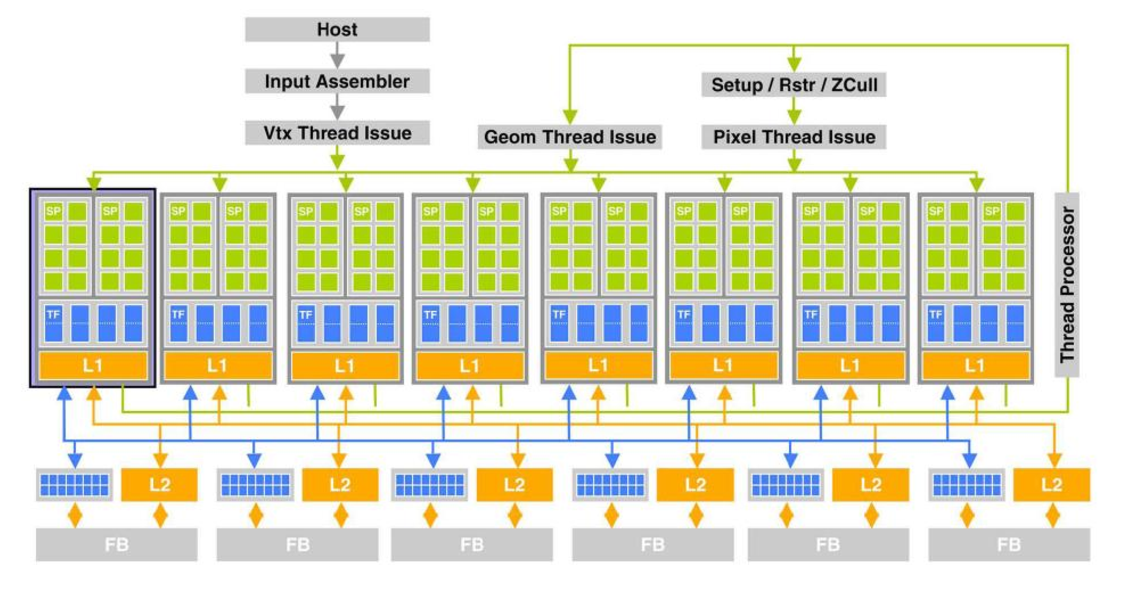
\includegraphics[height = 6cm]{./ifl/image_top.pdf}
%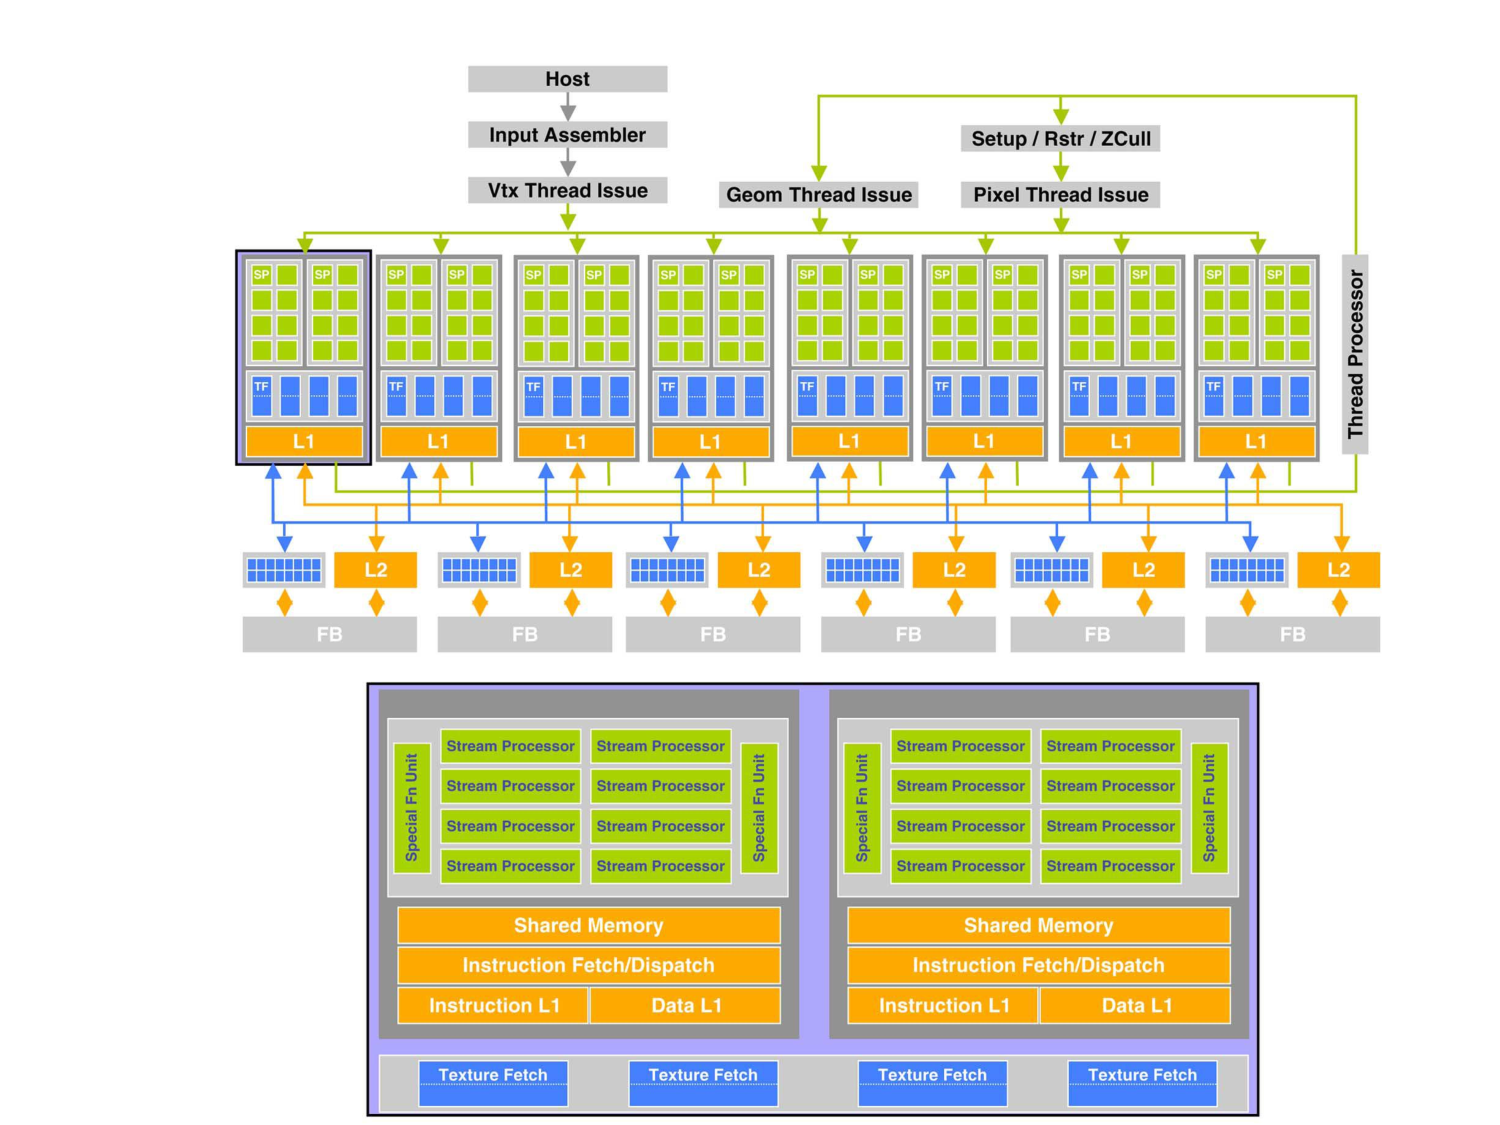
\includegraphics[width = 14cm]{image.pdf}
\caption{The NVIDIA 8800GTX GPU architecture, with 8 pairs of multiprocessors. Diagram courtesy of NVIDIA.}\label{fig:image}
\end{center}
\end{figure}


\noindent In CUDA, one writes a similar C function, called a {\em kernel},
to compute one element of the matrix. Then, the kernel is invoked as many
times as the matrix has elements, resulting in many threads, which can be
run in parallel. A predefined structure called {\tt threadIdx} is used to
label each of these many threads, and can be referred to in the kernel.
\begin{code}
// add 2 matrices on the GPU (simplified)
__global__ void addMatrix(float *a,float *b, float *c, int N)
{
  int i= threadIdx.x;
  int j= threadIdx.y;
  int index= i + j * N;
  c[index]= a[index] + b[index];
}

void main()
{
  // run addMatrix in 1 block of NxN threads:
  dim3 blocksize(N, N),
  addMatrix<<<1, blocksize>>>(a, b, c, N);
}
\end{code}
Here, a two dimensional {\em thread block} of size $N \times N$ is created.

CUDA uses {\em barrier synchronisation} and {\em shared memory} for
introducing communication between threads. Contents of shared memory (16kB
per multiprocessor in the architecture shown in Figure~\ref{fig:image}) is
visible to all threads in a thread block. It is very much faster to access
this shared memory than to access the global device memory. We shall see
later that Obsidian provides users with both shared and global arrays,
giving the user control over where data is to be stored.

Since many threads are now writing and reading from the same shared memory,
it is necessary to have a mechanism that enables the necessary
synchronisation between threads. CUDA provides a barrier synchronisation
mechanism called {\tt \_\_syncthreads()}. Only when all threads in a block
have reached this barrier can any of them proceed. This allows the
programmer to ensure safe access to the shared memory for the many threads
in a thread block.

Now, a {\em grid} is a collection of thread blocks. Each thread block runs
on a single multiprocessor, and the CUDA system can schedule these individual
blocks in order to maximise the use of GPU resources. A complete program
then consists not only of the kernel definitions, but also of code, to be
run on the CPU, to launch a kernel on the GPU, examine the results and
possibly launch new kernels. In this paper, we will not go into details
about how kernels are coordinated, but will concentrate on how to write
individual kernels, as this is the part of Obsidian that is most developed.
In Obsidian, we write code that looks like the Lava descriptions in
section~\ref{sec:combinators}, and we generate CUDA code like that shown
above. This is a considerably more complex process than the generation of
netlists in Lava.


           %% I decided to put a separate section on GPUs, rather
                       %% than trying to cover it in the intro.



\documentclass[3p,times]{elsarticle}

\usepackage{ecrc} % [headings]{espcrc1}

\volume{00}

\firstpage{1}

\journalname{Procedia Computer Science}

\jid{procs}

\jnltitlelogo{Procedia Computer Science}
%\setlength{\parindent}{0pt}
%\setlength{\parskip}{1ex plus 0.5ex minus 0.2ex} 



\usepackage{color}
\usepackage{graphicx}
\usepackage{subfigure}
\usepackage{placeins}
\usepackage[font=sf]{caption}
\usepackage[figuresright]{rotating}


% set the starting page if not 1
% \setcounter{page}{17}

% add words to TeX's hyphenation exception list
\hyphenation{author another created codependent financial paper re-commend-ed Post-Script}

%-------------------------------------------------------------------------------



%\title{Obsidian: GPU Computing Using Haskell (DRAFT)} 
%\author{Joel Svensson, Koen Claessen and Mary Sheeran} 
%\runauth{Joel Svensson, Koen Claessen and Mary Sheeran}

%% \date{\today} 

% \runtitle{Obsidian: GPU Computing Using Haskell}
\runauth{Joel Svensson, Koen Claessen and Mary Sheeran}

\begin{document}
\begin{frontmatter}

%% Title, authors and addresses

%% use the tnoteref command within \title for footnotes;
%% use the tnotetext command for the associated footnote;
%% use the fnref command within \author or \address for footnotes;
%% use the fntext command for the associated footnote;
%% use the corref command within \author for corresponding author footnotes;
%% use the cortext command for the associated footnote;
%% use the ead command for the email address,
%% and the form \ead[url] for the home page:
%%
%% \title{Title\tnoteref{label1}}
%% \tnotetext[label1]{}
%% \author{Name\corref{cor1}\fnref{label2}}
%% \ead{email address}
%% \ead[url]{home page}
%% \fntext[label2]{}
%% \cortext[cor1]{}
%% \address{Address\fnref{label3}}
%% \fntext[label3]{}

\dochead{}
%% Use \dochead if there is an article header, e.g. \dochead{Short communication}

\title{GPGPU Kernel Implementation and Refinement using Obsidian}

%% use optional labels to link authors explicitly to addresses:
%% \author[label1,label2]{<author name>}
%% \address[label1]{<address>}
%% \address[label2]{<address>}

\author{Joel Svensson}
\author{Koen Claessen}
\author{Mary Sheeran}
%\affiliation{Chalmers University of Technology}

\address{CSE Dept., Chalmers University of Technology, Gothenburg, Sweden} 

\begin{abstract}
Obsidian is a domain specific language for data-parallel programming 
on graphics processors (GPUs). It is embedded in the functional 
programming language Haskell. The user writes code using constructs 
familiar from Haskell (like {\tt map} and {\tt reduce}), recursion 
and some specially designed combinators for combining GPU programs. 
NVIDIA CUDA code is generated from these high level descriptions, and 
passed to the {\tt nvcc} compiler~\cite{CUDAGuide2.0}. Currently, we 
consider only the generation of single kernels, and not their coordination.

This paper is focussed on how the user should work with Obsidian, 
starting with an obviously correct (or well-tested) description of the 
required function, and refining it by the introduction of constructs to 
give finer control of the computation on the GPU. For some combinators, 
this approach results in CUDA code with satisfactory performance, promising 
increased productivity, as the high level descriptions are short and 
uncluttered. But for other combinators, the performance of generated code 
is not yet satisfactory. Ways to tackle this problem and plans to integrate 
Obsidian with another higher-level embedded language for GPU programming in 
Haskell are briefly discussed.




%Obsidian is a domain specific language for Data-parallel 
%programming on graphics processors (GPUs) embedded in Haskell. 
%From high level descriptions, code for execution on a GPU is generated.
%Obsidian generates NVIDIA CUDA code that is passed to the {\tt nvcc} 
%compiler \cite{CUDAGuide2.0}. 

%This paper is mainly focused on the usage of Obsidian. The implementation
%of Obsidian itself and a discussion of how the CUDA code is generated can 
%be found in \cite{JSTECH}.



%\vspace{1pc}
\end{abstract}

\begin{keyword}
%% keywords here, in the form: keyword \sep keyword
Data-parallel \sep Embedded language \sep GPUs \sep Haskell  
%% PACS codes here, in the form: \PACS code \sep code

%% MSC codes here, in the form: \MSC code \sep code
%% or \MSC[2008] code \sep code (2000 is the default)

\end{keyword}

\end{frontmatter}


%-------------------------------------------------------------------------------
\section{Introduction} 

Multicore and manycore processors are becoming increasingly common. Modern 
graphics processing units (GPUs) are examples of manycore processors. Today 
GPUs come with hundreds of processing elements capable of managing thousands 
of threads \cite{Brief8800}. The Obsidian project is about exploring ways 
to program these new machines.  

Obsidian is a domain specific language for general purpose programming on 
GPUs (GPGPU), capable of generating code for modern NVIDIA GPUs. 
In~\cite{JSMSKC_IFL08} we describe a version of Obsidian that uses a monadic 
interface. In the current version of Obsidian the monad has been replaced 
by another data structure, closely related to Arrows~\cite{Arrows}, representing GPU programs. Although the details are 
left out because of space limitations, the use of this GPU program representation 
can be seen in section~\ref{sec:GPUPrograms}. For a description of the implementation 
see~\cite{JSTECH} and for more general information on embedded language 
implementation see~\cite{Elliott03:CompileDSEL-JFP}.

GPU design is driven by the performance demands of graphics applications. 
The kind of processing that is common in graphics falls in the data-parallel 
category \cite{GEMS2}.
% One example of a computation from graphics is the 
%transformation of vertices between different coordinate systems. That is, 
%each vertex is multiplied by the same transformation matrix, fitting  the 
%data-parallel paradigm perfectly. 



%-------------------------------------------------------------------------------
\subsection{NVIDIA GPUs and CUDA}


Starting with the 8000 series of GPUs (the G80 architecture), NVIDIA's 
GPUs came with a unified architecture, meaning that all the 
processing elements on the GPU are of the same kind. This was different from 
the previous generation's GPUs, which typically had two kinds of 
processing elements, fragment and vertex processors.  
%There was one kind of processor designed to process fragment/pixel programs and another to process vertex data. 
Now these two kinds 
of processors are replaced by a single kind with capabilities surpassing both 
of the old ones. This new unified architecture together with development tools 
for GPGPU programming go under the 
name CUDA (Compute Unified Device Architecture) 
\cite{CUDAGuide2.0}. CUDA offers the GPGPU programmer a C %,wwwcuda,Brief8800
compiler and libraries for CUDA enabled GPUs (NVIDIA 8000 series and above).  

Figure~\ref{fig:gpu}, shows a conceptual picture of a CUDA enabled GPU. The GPU 
has a number of {\em Multiprocessors} (MP in the picture). These MPs contain 
a number of small processing elements called {\em Streaming Processors} (SP). 
These SPs operate in an SIMD fashion. All SPs in a given MP execute 
the same instruction each clock cycle. 

Each MP is capable of maintaining a large number of threads in flight at the 
same time. A group of threads running on an MP is referred to as a {\em block}. 
A block can contain more threads then there are processing elements; today a 
block can hold up to 1024 threads. There is a scheduler mapping these threads 
over the SPs available. Threads are scheduled in groups called {\em warps} 
consisting of 32 threads that are executed in an SIMD fashion on the MPs.
Conditionals that take different paths within a warp have a negative effect 
on performance; the two diverging paths will in fact be executed sequentially 
\cite{BestPrac}.
%There are however, more threads in a
%warp then there are SPs, so the SPs are switching threads to work on 
%between every instruction. This means that conditionals that
%take different paths within a warp have a negative effect on performance;
%the two diverging paths will in fact be executed sequentially \cite{BestPrac}. 



The MPs also have local memory that is shared between all the 
SPs of that MP, and thus referred to as {\em Shared Memory} in the figure. 
It can be used to exchange information between threads running 
on the SPs; it can also be used as a software managed cache. 
Threads within a warp can safely communicate using shared memory without 
the need for any synchronisation. Threads from different warps, however, need 
to use a synchronisation primitive to ensure a coherent view of the shared 
memory. In CUDA C this primitive is called {\tt \_\_syncthreads()}. The
{\tt \_\_syncthreads()} primitive provides a barrier that all threads of a 
block must reach before any is allowed to proceed. 

The {\em Global memory} is located off chip and is accessible by all MPs. 
In current GPUs, accesses to this memory are uncached.


\begin{figure}
\begin{center}
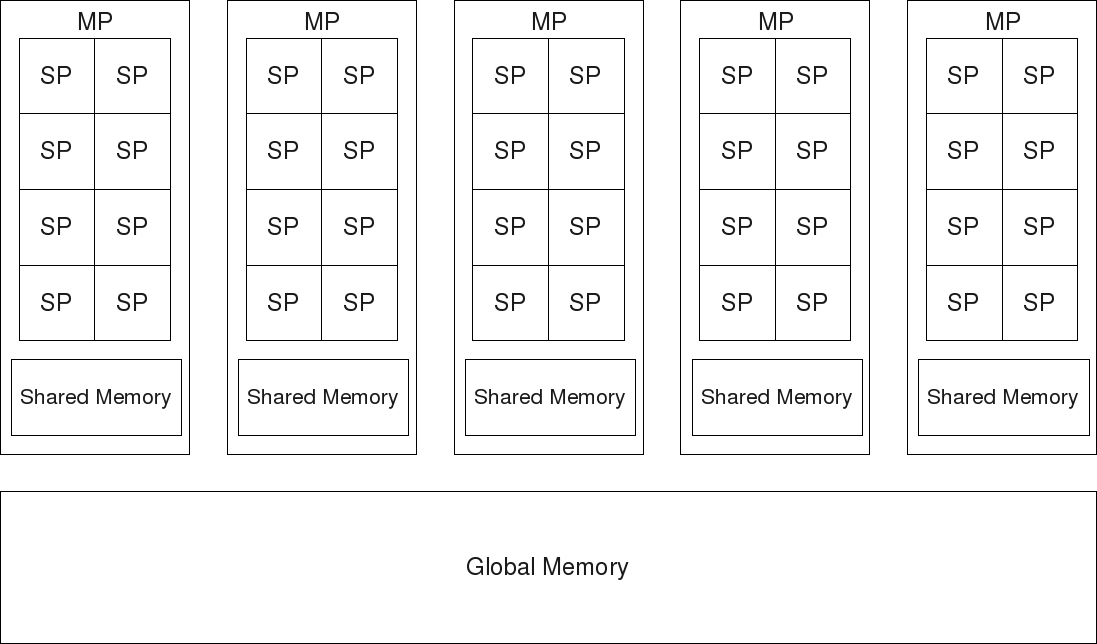
\includegraphics[width=.65\linewidth]{./pictures/gpu.jpg}
\caption{Conceptual image of a CUDA enabled GPU.}
\label{fig:gpu}
\end{center}
\end{figure}

\FloatBarrier

% ------------------------------------------------------------------------------
\subsection{Aims of Obsidian}

The initial goal of Obsidian is to simplify the development of GPU kernels, 
the building blocks of larger GPU programs. In the future, ways to combine 
kernels into larger algorithms will also be explored. 

When implementing an algorithm in CUDA, what to compute and how to compute it 
become codependent. Choices such as how many elements the kernel operates on 
and how many threads it uses affect each other greatly. Once a kernel 
is designed with a particular number of elements per thread, this becomes hard to tweak. In CUDA the programmer writes a single program 
parameterised over a thread identity. This program is then executed by 
several threads. Taking this point of view often means that what elements to use 
needs to be computed from the threadIDs. Coming up with these indexing 
computations is not always trivial. 

In Obsidian the program is described as 
a computation between arrays, and combinators are used instead of direct indexing 
into structures. 
Obsidian provides an environment where it is easy to experiment with different
partitionings and choices when implementing an algorithm. It is 
possible to write a simple running first prototype version of a kernel 
without thinking about architectural details. The prototype implementation 
can then be refined into a more efficient implementation. 
The aim of Obsidian is to raise the level of abstraction for the GPGPU 
programmer and to relieve the programmer of details such as laying things out 
in memory. Performance affecting decisions should be easy to make 
and change without major rewrites of the code.



%-------------------------------------------------------------------------------
\section{Programming in Obsidian} 

Obsidian is a language for GPGPU programming embedded in Haskell. Many of 
the language features resemble those of Lava, a hardware description and 
verification language \cite{lavaICFP}. The justification to use language 
constructs similar to that of a hardware description language came from 
the observation that GPGPU algorithms often were explained using circuit-like 
pictures, see for example \cite{GEMS3}. 

%Obsidian can be used to describe hardware like algorithms. These are algorithms
%where the number of inputs and outputs are fixed, not dependent on 
%the values of inputs. 
%There are a large number of algorithms falling into this category. For example, 
%there are numerous sorting algorithms (sorting networks) and parallel prefix 
%algorithms implementable in this way. Also, there are examples in the 
%literature where GPGPU programmers implement their kernels to operate on very 
%specific array sizes \cite{GEMS3}. In a later stage, when the kernels are 
%composed into algorithms on large arrays, support for variable length 
%arrays is introduced.

Obsidian can be explained as two sub-languages. First there is a language of 
arrays and operations on arrays, and second, a language that enables mapping of the 
array language programs onto the GPU. 
 
%-------------------------------------------------------------------------------
\subsection{Array Language}
\label{sec:ArrayLanguage}
\FloatBarrier
Arrays in Obsidian do not, like in C, name an area of memory. Instead, an 
array is represented by an abstract data type, called {\tt Arr}, supporting 
the following operations: {\tt (!)} for indexing, {\tt len} 
returns the length of an array and {\tt mkArr} that given a function from 
indexes to elements and a length gives an array. For example using these 
operations reversing an array can be accomplished as follows: 

\begin{small}
\begin{verbatim}
rev :: Arr a -> Arr a 
rev arr  = mkArr ixf n
    where 
        ixf ix = arr ! (fromIntegral (n-1) - ix)
        n = len arr 
\end{verbatim}
\end{small}
\noindent
Array reversal is polymorphic in the element type which gives the {\tt rev} 
program the type {\tt Arr a -> Arr a}. 
Internally an array is represented by the computation that gives its elements. 
The array type consists of two parts, a function from indices to elements and an 
integer representing its length:
%-------------------------------------------------------------------------------
\begin{small}
\begin {verbatim} 
data Arr a = Arr (IndexE -> a) Int 
\end{verbatim}
\end{small}
%-------------------------------------------------------------------------------
%An array is a function from an index expression, {\tt IndexE}, to elements.
\noindent 
The length of the array is static, known at compile time, and is represented
by an {\tt Int}. The elements of an array can be {\tt Int}, {\tt Float} or 
{\tt Bool} valued expressions, represented by the types {\tt IntE}, 
{\tt FloatE} and {\tt BoolE}. Arrays can also contain arrays and tuples 
as elements. 

Obsidian provides a number of functions on this array type. For example, 
a function can be mapped over an array using {\tt fmap}. 
%see figure~\ref{fig:zipunzip}:

%-------------------------------------------------------------------------------
\begin{small}
\begin{verbatim}
fmap :: (a -> b) -> Arr a -> Arr b
\end{verbatim}
\end{small}
%-------------------------------------------------------------------------------
\noindent
The array type is also an instance of {\tt Foldable}, so there is a function 
{\tt foldr} (often called {\tt reduce}) defined on arrays: 

\begin{small}
\begin{verbatim}
foldr :: (a -> b -> b) -> b -> Arr a -> b
\end{verbatim}
\end{small}
\noindent
Two other basic functions on arrays that are available are {\tt pair} and 
{\tt unpair}: 
\begin{small}
\begin{verbatim}
pair :: Arr a -> Arr (a,a)
unpair  :: Choice a => Arr (a,a) -> Arr a
\end{verbatim}
\end{small}
\noindent
The function {\tt pair} takes an array and returns an array of pairs where 
the first element of the input array is paired up with the second, the 
third with the forth and so on. The {\tt unpair} function does the 
opposite. % see figure~\ref{fig:pairunpair}.

The {\tt Choice} class contains those types that have an {\tt ifThenElse} 
function defined on them:  
\begin{small}
\begin{verbatim}
ifThenElse :: Choice a => BoolE -> a -> a -> a
\end{verbatim}
\end{small}
\noindent
Another example of a function given in the array library is {\tt zipp} of type{\tt (Arr a, Arr b) -> Arr (a, b)}.
%\begin{small}
%\begin{verbatim}
%zipp :: (Arr a, Arr b) -> Arr (a, b)
%\end{verbatim}
%\end{small}
This function performs on arrays what the normal Haskell {\tt zip} 
does on lists. However, the input to {\tt zipp} is a pair of arrays. 

%Array programs like those described here make up the building blocks used
%to form larger GPU programs. How to create a GPU program from these is 
%shown in the following section. 


%-------------------------------------------------------------------------------

%\FloatBarrier
\subsection{GPU Programs}
\label{sec:GPUPrograms}

The second layer of Obsidian offers a data type that represents a GPU program
with input {\tt a} and output {\tt b}:

\begin{small}
\begin{verbatim} 
data a :-> b = ... 
\end{verbatim}
\end{small} 
\noindent
%The details of {\tt a :-> b} are shown in section~\ref{sec:Implementation}. 
\noindent
Informally we can think of {\tt a\nolinebreak~:->\nolinebreak~b} as representing programs that operate 
as illustrated in figure~\ref{fig:program}. This figure 
shows a program that performs some computation using a number of threads 
followed by a barrier synchronisation, and so on. The contents of the 
boxes marked with {\em Pure} can be thought of as containing an array 
program.% such as those in section~\ref{sec:ArrayLanguage}.
The type constructor {\tt :->} is a variant of an arrow, which in turn is a generalisation of a monad~\cite{JSTECH}.
%
\begin{figure}
\begin{center}
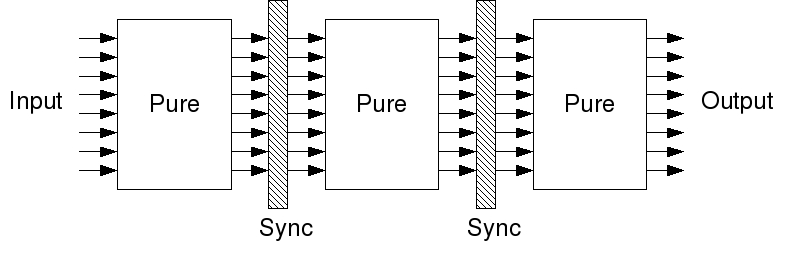
\includegraphics[width=.60\linewidth]{./pictures/prg_intuit.jpg}
\caption{A GPU program of type  {\tt a :-> b} can be thought 
of as pure computations interspersed by syncs.}
\label{fig:program}
\end{center}
\end{figure}
\noindent
One way to create a GPU program is by using the function {\tt pure} of type {\tt (a -> b) -> a :-> b}.
%\begin{small}
%\begin{verbatim}
%pure :: (a -> b) -> a :-> b
%\end{verbatim}
%\end{small}
For example the array language program {\tt fmap (+1)}, that increments 
every element of an array, can be lifted to a GPU program: 
%
\begin{small}
\begin{verbatim}
incr :: Arr IntE :-> Arr IntE 
incr = pure $ fmap (+1)
\end{verbatim}
\end{small} 
 \noindent
GPU programs can be executed on the GPU from
{\em GHCi} (the Haskell interpreter) using the function {\tt execute}: 

\begin{small}
\begin{verbatim}
execute :: (Flatten a, Flatten b) => (Arr a :-> Arr b) -> [a] -> IO [b]
\end{verbatim}
\end{small}
\noindent
%The class {\tt Flatten} will be explained in detail in 
%section~\ref{sec:Implementation}, but 
Instances of {\tt Flatten} are all the types that can be stored in the 
GPU memory. Examples of types that are in {\tt Flatten} are {\tt IntE}, 
{\tt FloatE}, {\tt BoolE}. Arrays and pairs of things that are in Flatten 
are also instances of {\tt Flatten}.
Here, {\tt execute} is used in order to run an instance of the {\tt incr} 
program on the GPU:

\begin{small}
\begin{verbatim}
*Obsidian> execute incr [0..9]
[1,2,3,4,5,6,7,8,9,10]
\end{verbatim}
\end{small}
\noindent
The elements of the Haskell list given to {\tt execute} are used to create 
an input array to the kernel. Following this, the kernel is executed on the
GPU and the result is read back and presented as a Haskell list. 

In the example above, the {\tt execute} function generates the following kernel 
corresponding to the given GPU program:
\begin{small}
\begin{verbatim}
__global__ void generated(word* input,word* result){
  unsigned int tid = (unsigned int)threadIdx.x;
  extern __shared__ unsigned int s_data[];
  word __attribute__((unused)) *sm1 = &s_data[0];
  word __attribute__((unused)) *sm2 = &s_data[0];
  ix_int(result,tid) = (ix_int(input,tid) + 1);
}
\end{verbatim}
\end{small}
\noindent
The generated kernel has two arguments, an input array of words and an 
output array of words. Words represent 32-bit quantities that can be either
floating point or integer valued. This particular kernel does not use 
any shared memory; the incremented values are stored directly into the 
result array that resides in global memory.  

Given two GPU programs, {\tt f} and {\tt g}, of suitable types, a 
composite GPU program can be created by passing the output of {\tt f} to the 
input of {\tt g}. In Obsidian this is done using the composition operator (or combinator)
{\tt (->-)}: 


\begin{small}
\begin{verbatim}
(->-) :: (a :-> b) -> (b :-> c) -> (a :-> c)
\end{verbatim}
\end{small}
\noindent
The following illustrates the use of {\tt (->-)} by implementing a 
program that increments every element of an array but also reverses 
the array: 

\begin{small}
\begin{verbatim}
increv :: Arr IntE :-> Arr IntE 
increv = pure (fmap (+1)) ->- pure rev

*Obsidian> execute increv [0..9]
[10,9,8,7,6,5,4,3,2,1]
\end{verbatim}
\end{small}
\noindent
The code generated from the {\tt increv} program is very similar to that 
of {\tt inc} but the indexing is reversed:

\begin{small}
\begin{verbatim}
__global__ void generated(word* input,word* result){
  unsigned int tid = (unsigned int)threadIdx.x;
  extern __shared__ unsigned int s_data[];
  word __attribute__((unused)) *sm1 = &s_data[0];
  word __attribute__((unused)) *sm2 = &s_data[0];
  ix_int(result,tid) = (ix_int(input,(9 - tid)) + 1);
}
\end{verbatim}
\end{small}
\noindent
The code generated for the {\tt incr} and {\tt increv} examples uses 
$10$ threads to compute the resulting array. By default, the result will 
be computed using a number of threads equal to the number of elements in 
the return array. 

The {\tt increv} program can also be specified with an explicit storing 
of intermediate values between the {\tt rev} and the {\tt fmap (+1)}. 
This is accomplished using a primitive GPU program called {\tt sync}:

\begin{small}
\begin{verbatim}
sync  :: Flatten a => Arr a :-> Arr a

increv :: Arr IntE :-> Arr IntE 
increv = pure (fmap (+1)) ->- sync ->- pure rev
\end{verbatim}
\end{small} 
\noindent
This version of {\tt increv} computes the same result as the previous one. 
However, it does so by computing {\tt fmap (+1)} on the array, storing the
intermediate result in shared memory followed by computing the reverse.
The CUDA C code for this version of {\tt increv} looks like this. Notice 
how the shared memory is used and the call to {\tt \_\_syncthreads()}: 
%
\begin{small}
\begin{verbatim}
__global__ void generated(word* input,word* result){
  unsigned int tid = (unsigned int)threadIdx.x;
  extern __shared__ unsigned int s_data[];
  word __attribute__((unused)) *sm1 = &s_data[0];
  word __attribute__((unused)) *sm2 = &s_data[8];
  ix_int(sm1,tid) = (ix_int(input,tid) + 1);
  __syncthreads();
  ix_int(result,tid) = ix_int(sm1,(7 - tid));
}
\end{verbatim}
\end{small}


\section{Outline of Code Generation}
\label{sec:CodeGen}
\FloatBarrier

This section briefly reviews the code generation process using 
a hyphothetical program as example. The program under consideration 
is this: 

\begin{small}
\begin{verbatim}
prg = pure (fmap f) ->- sync -> rev ->- sync ->- pure (fmap g) 
\end{verbatim}
\end{small}

This program applies some function {\tt f} to all elements of 
an array. The array is then reversed and lastly a function {\tt g} 
is applied to all elements. Between every operation there is a {\tt sync}.
The program {\tt prg} is an element of the datatype {\tt (a :-> b)}. 
To see what happens during code generation, it is necessary to know 
the implementation of this type.
\begin{small}
\begin{verbatim} 
data a :-> b 
   = Pure (a -> b) 
   | Sync (a -> Arr FData) (Arr FData :-> b) 
\end{verbatim}
\end{small} 
\noindent
The type {\tt (a :-> b)} is essentially a list of computations. The 
function {\tt pure} is directly implemented using the constructor 
{\tt Pure}. The function {\tt sync} is implemented in terms of the 
constructor {\tt Sync}:

\begin{small}
\begin{verbatim} 
sync :: Flatten a => (Arr a :-> Arr a)
sync = Sync (fmap toFData) (pure (fmap fromFData))
\end{verbatim}
\end{small} 
\noindent
The example program {\tt prg} would be represented as follows: 
%
\begin{small}
\begin{verbatim} 
Sync (fmap (toFData . f)) (Sync ((fmap toFData) . rev . (fmap fromFData)) (Pure (fmap g)))   
\end{verbatim}
\end{small} 
\noindent
From this representation, which is essentially the list {\tt [fmap f, rev, fmap g]},
the CUDA code is generated as outlined in figure~\ref{fig:codegen}. 
An input array is created and applied to the first stage of the computation, 
{\tt (fmap f)}, resulting in: 
\begin{small}
\begin{verbatim}
Arr (\ix -> f(index (variable ``input'') ix)) n. 
\end{verbatim}
\end{small}

The information given by this array is used to construct the C assignment 
statement {\tt sm1[tid] = f(input[tid])} as seen in the figure.

Following this a new Obsidian level array that indexed into {\tt sm1} is 
created and used as input to the second stage of the computation. 

%Following this a new Obsidian level array that looks as follows is created: 
%\begin{small}
%\begin{verbatim}
%Arr (\ix -> index (variable ``sm1'') ix) n. 
%\end{verbatim}
%\end{small}



%This expression is used to generate a 
%C assignment. The array is stored into one of two shared memory arrays 
%This array  is used as input to the next phase. The computation is then double 
%buffered between the two shared memory arrays. 
%giving an expression.


\begin{figure}
\begin{center}
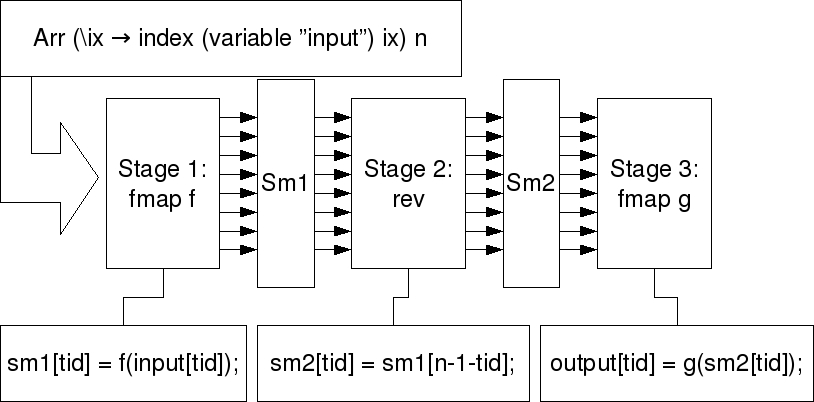
\includegraphics[width=.65\linewidth]{./pictures/codegenexample.jpg}
\caption{Outline of the code generation procedure.}
\label{fig:codegen}
\end{center}
\end{figure}


%-------------------------------------------------------------------------------

\section{Case Studies}
\label{sec:CaseStudies}

\FloatBarrier
This section describes a few slightly larger Obsidian programs. The main purpose of this section is to show 
how we want to write GPGPU programs using Obsidian. 
%How the performance 
%of the generated code can be improved is discussed in section~\ref{sec:FutureWork}  
%%% Move this later.  XXX

\subsection{Sorting}

Sorting is a popular function to place on the GPU, see~\cite{SORT1,SORT3}.
{\em Odd-Even merge sort}, due to Batcher, uses a merger component called the Odd-Even merger. This 
merger merges two sorted arrays. In Obsidian this merger and sorter 
can be implemented using the combinators {\tt two}, {\tt ilv}, {\tt evens}
and {\tt odds}. For a detailed description of these combinators see
~\cite{lavaSorter}.

\begin{small}
\begin{verbatim}
mergeOE :: (Choice a, Flatten a) => Int -> ((a,a) -> (a,a)) -> (Arr a :-> Arr a)
mergeOE 1 f = pure (evens f)
mergeOE n f = ilv (mergeOE (n-1) f) ->- sync ->- pure (odds f)
\end{verbatim}
\end{small}
\noindent
This is actually a pattern into which any two-input two-output function
can be plugged. However, we choose the following {\em comparator} function (a compare and swap operation). The resulting merger can be executed on the GPU.
\begin{small}
\begin{verbatim}
cmp :: (Ordered a, Choice (a, a)) => (a, a) -> (a, a)
cmp (a,b) = ifThenElse (a <* b)  (a,b) (b,a)

*Obsidian> execute GPU (mergeOE 3 cmp) ([1,3,5,7,2,4,6,8] :: [IntE]) 
[1,2,3,4,5,6,7,8]
\end{verbatim}
\end{small}
\noindent
Given this merger, the sorter is implemented by recursively sorting 
two halves of the input array followed by an application of the merger:

\begin{small}
\begin{verbatim}
sortOE :: Int -> (Arr IntE :-> Arr IntE)
sortOE  0 =  pure id
sortOE  n =  two (sortOE (n-1)) ->- sync ->- mergeOE n cmp 

*Obsidian> execute GPU (sortOE 3) [6,0,1,3,4,2,5,7]
[0,1,2,3,4,5,6,7]
\end{verbatim}
\end{small}

The performance of the code generated from this sorter specification is poor. It
runs about three times slower than the example Bitonic
sorter distributed with the CUDA SDK. 
The reason is that nested applications of the {\tt two} and {\tt ilv} 
combinators are hard to optimise. We expect that single (parameterised) combinators corresponding
to particular nestings of these combinators will bring significant performance improvement.
%
%The reason for the poor performance in this case is the code 
%condition of the code generated from the deep nestling of applications of 
%{\tt two} and {\tt ilv} that the code generator currently does a very bad job 
%at optimising. There may be alternative ways to implement these combinators 
%or entirely different ones should replace them. 


%-------------------------------------------------------------------------------
\subsection{Parallel Prefix}
\FloatBarrier

This subsection shows the implementation of a parallel prefix (also called scan) 
kernel, known as {\tt sklansky} after J. Sklansky \cite{Sklansky:1960:CSA}.
This kernel will then be optimised step-by-step using Obsidian. This 
optimisation effort uses an experimental feature of Obsidian called {\tt syncHow}. 
This is different from the normal {\tt sync} in the way it assigns work to threads. 
For a more thorough explanation of {\tt syncHow} see ~\cite{JSTECH}.
For an explanation of the parallel-prefix operation see~\cite{BlellochTR90}. 

The sklansky parallel prefix algorithm 
is implemented by splitting the inputs in two halves and recursively 
applying sklansky to both halves. The two sub-results are then 
joined by applying the operation between the highest index of the first
sub-result and all the elements in the second sub-result, this is done 
using a function called {\tt fan}: 

\begin{small}
\begin{verbatim}
fan op arr = conc (a1, (fmap (op c) a2)) 
    where (a1,a2) = halve arr
          c       = a1 ! (fromIntegral (len a1 - 1))
\end{verbatim}
\end{small}
\noindent
The {\tt sklansky} function is now implemented using 
{\tt two} and {\tt fan}: 

\begin{small}
\begin{verbatim}
sklansky :: (Flatten a, Choice a) => Int -> (a -> a -> a) -> (Arr a :-> Arr a) 
sklansky 0 op = pure id
sklansky n op = two (sklansky (n-1) op) ->- pure (fan op) ->- sync
\end{verbatim}
\end{small}

Executing ({\tt sklansky 3 (+)}) on the GPU given input {\tt [0..7]} computes
the prefix sum as expected, returning {\tt [0,1,3,6,10,15,21,28]} 
%Executing a small instance of the prefix network above on the GPU has 
%the following result: 

%\begin{small}
%\begin{verbatim}
%*Obsidian> execute (sklansky 3 (+)) ([0..7] :: [IntE])
%[0,1,3,6,10,15,21,28]
%\end{verbatim}
%\end{small}

If {\tt sklansky} is used to generate code for an array of 512 elements,
it uses 512 threads to calculate the prefix sums. However, the number of 
applications of the {\tt op} operator that is needed in any stage of the 
algorithm is only 256. This indicates that 
using 256 threads to compute the result would give more efficient
use of the GPU's resources.

Since the code generated by Obsidian is not by default {\em in-place} with regard 
to shared memory, each thread in the 256 threaded program needs to both perform 
the operation between two elements and copy one value unchanged. This is desired
because then each thread performs the exact same operations,
which means that there is no risk for divergence within a warp. 

This perfect division of labour is not obtainable with the current 
implementation of the {\tt How} argument to {\tt sync}. However, one 
division of the work that has experimentally been shown to perform well, see 
table in next section,  
is to let each thread $tid$ perform the work of $tid$ and $tid + 256$. This 
program is shown below: 

\begin{small}
\begin{verbatim}
sklansky1 :: (Flatten a, Choice a) => Int -> (a -> a -> a) -> (Arr a :-> Arr a) 
sklansky1 0 op = pure id
sklansky1 n op = two (sklansky1 (n-1) op) ->- pure (fan op) ->- syncHow (pairNth 256) 
\end{verbatim}
\end{small}


Another optimisation to apply to the sklansky algorithm is the removal of 
unnecessary {\tt \_\_syncthreads()} calls from the generated code, this is 
done by using {\tt syncWarp}. It is up to the programmer to ensure that it 
is safe to use {\tt syncWarp}. For a sklansky network of size 32, it should 
be safe to leave out the {\tt \_\_syncthreads} since all of the communication 
stays within a warp. Using this information leads to the following code where 
the sklansky networks of size 32 or smaller use {\tt syncWarpHow}.


\begin{small}
\begin{verbatim} 
sklansky2 :: (Flatten a, Choice a) => Int -> (a -> a -> a) -> (Arr a :-> Arr a) 
sklansky2 0 op = pure id
sklansky2 n op = two (sklansky2 (n-1) op) ->- pure (fan op) 
                   ->-  if n <= 5 
                         then syncWarpHow (pairNth 256)
                         else syncHow (pairNth 256)
\end{verbatim}
\end{small}

%% XXX Why is there no explicit 32 anywhere in the vicinity of SyncWarpHow?

A last tweak to force the algorithm to compute {\em in-place}. This 
is accomplished using the primitives {\tt syncIP} and {\tt syncIPHow}, which
are variants of {\tt sync} that enforce {\em in-place} computation.

%-------------------------------------------------------------------------------
\subsubsection{Parallel Prefix Sums on large arrays}
\FloatBarrier

The Sklansky kernels given above can be used in an algorithm that computes 
the parallel prefix of a large array. This is done in the same way as in
~\cite{harris07parallel}.
The table below shows the results of using the different parallel prefix 
kernels from above in an algorithm for computing the prefix sums of 
$2^{20}$ elements.

\begin{small}
\begin{center}
  \begin{tabular}{  l | r | r |r | r  }
    %\hline
    Kernel          & In-place & Sync in Warp & Threads & ms   \\ \hline
    NVIDIA SDK      & Yes      & N/A          & 256     & 0.64 \\
    Hand Optimised  & Yes      & No           & 256     & 0.74 \\ 
    sklansky        & No       & yes          & 512     & 1.06 \\ 
    sklansky1       & No       & yes          & 256     & 0.89 \\ 
    sklansky2       & No       & No           & 256     & 0.86 \\ 
    sklansky3       & Yes      & No           & 256     & 0.79 \\
    %\hline
  \end{tabular}
\end{center}
\end{small}

The table above shows the running times of six different Sklansky kernels. 
All runtime measurements where performed on an NVIDIA 9800GX2 using one GPU. 
The code labeled {\em Hand Optimised} was written directly in CUDA. 
This kernel was the result of two afternoons of optimisation effort by 
two people. The three following kernels {\em sklansky} to {\em sklansky2} are 
generated from the given Obsidian programs. The version called {\em sklansky3} 
is identical to {\tt sklansky2} except is in-place. Even the very first version, 
{\em sklansky} performs reasonably well, but by using the experimental features 
the performance can be pushed quite close to the hand optimised version.  
The fastest kernel, called {\em NVIDIA SDK}, is the one supplied 
with the CUDA SDK. This kernel is based on the Brent-Kung network and its 
implementation is shown in~\cite{harris07parallel}. The {\tt NVIDIA SDK} 
kernel is highly optimized with regards to its memory access pattern and 
so the code is considerably more complicated than that of any of the Obsidian parallel-prefix kernels.
 

%-------------------------------------------------------------------------------
\FloatBarrier
\section{Future work}
\label{sec:FutureWork}

Obsidian is work in progress and as such it changes a lot. Future work will both
explore improvements to code generation for kernels and ways to coordinate kernels.

In order to get to the quite efficient version of the {\tt sklansky} kernel 
in section~\ref{sec:CaseStudies}, the experimental {\tt How} argument to {\tt sync} was needed. 
This needs to be 
explored further. {\tt How} as it is today, any function of type
{\tt IndexE -> [IndexE]}, offers too much freedom and with that the risk of
introducing errors. We are searching for an elegant model for expressing how and what 
to compute, and for ways to integrate this with
the language. This is our biggest research challenge.

Section~\ref{sec:CaseStudies}, on case studies, showed that it is possible to
generate quite efficient code from Obsidian programs. The current version 
generates efficient code for very specific uses of the {\tt two} combinator, 
for example the kind used in the {\tt sklansky} parallel prefix network. More 
work needs to be done in order to find a good way to produce efficient code 
for a larger set of combinators. 
This may very well involve designing new combinators that do not need
to be nested as the current ones do.

The CUDA code generated by Obsidian uses very few registers. In fact,
the generated code is under-utilizing the resources of the GPU. The generated 
code also contains many common subexpressions. This hints that applying a 
step of common subexpression elimintaion would be beneficial, increasing 
the register use and reducing the repeated computation of values. Performing
common subexpression elimination would also lower the instruction count,
which is quite high to begin with, because loops are unrolled. 
The register usage and instruction count values on which these conclusions 
are based where obtained using the CUDA profiler supplied as part of the 
CUDA toolkit~\cite{wwwcuda}.

Obsidian can currently only be used to generate kernels, the small 
building blocks used to form larger GPU algorithms. As future work, 
methods of describing kernel coordination in a high level fashion will 
be investigated.

At the University of New South Wales, Manuel Chakravarty 
et. al. are developing another language for GPGPU programming
called Accelerate. Accelerate is also embedded in Haskell, but intends
to be at a higher 
level of abstraction than Obsidian. Accelerate supplies the programmer 
with a collection of basic building blocks for data parallel programming. 
Amongst these building blocks are {\tt map}, {\tt zipWith} and {\tt scan}.
With the Accelerate team at UNSW, we are looking into 
ways of combining the two complementary approaches. In this setting Obsidian 
could be used to generate the underlying kernels (the building blocks) that the Accelerate 
programmer uses to build a GPGPU application. 

A limitation of Obsidian is the inability to express algorithms where 
the length of the output array is dependent on the input data. 
An example of such a data dependent algorithm is {\tt filter}. The {\tt filter} 
function takes a sequence of elements and a predicate and produces a sequence 
of those elements for whom the predicate holds. Future work 
will also consist of searching for a suitable minimal language construct
to add that enables expressing such algorithms. 






%-------------------------------------------------------------------------------
\section{Related work}

GPUs are becoming more and more interesting to use in non-graphical applications.
A modern GPU is a manycore machine with, today, hundreds of processing elements. 
The question of how to program these machines arises. NVIDIA's answer is CUDA
\cite{CUDAGuide2.0}. CUDA supplies a slightly extended version of C in which 
the programmer can specify GPU kernels and the controlling CPU program in the 
same language. In CUDA the programmer writes a single program parameterised 
over a thread identity. Compare this to Obsidian where the program describes 
a computation over an array. 

There are a number of other C/C++ based languages that target 
GPGPU programmers, for example Brook\cite{Brook} and 
RapidMind\cite{RapidMind}. Brook, CUDA and RapidMind are major improvements from 
what was previously available for the programmer interested in general purpose 
computations on the GPU. 
%Before these, the GPGPU programmer only had the 
%graphics API to work with and needed to translate his or her programs into 
%graphics vocabulary in order to use the GPU. 

Higher level approaches are also being investigated. PyGPU embedds a GPGPU 
programming language in Python\cite{PyGPU}. PyGPU makes use of Python's 
introspective abilities to generate efficient code. 

Like Obsidian, Accelerate is embedded in Haskell \cite{GPUGEN}. Accelerate 
however, is higher level language than Obsidian. Where the purpose of 
Obsidian is to implement basic algorithmic building blocks such as 
reductions and prefix sums, Accelerate provide these building blocks as 
primitives. 

Vertigo is another GPU programming language embedded in Haskell\cite{Vertigo}.
Vertigo can be used to describe procedureal surfaces and textures and generates
efficient DirectX9 shader code. 

There are also many examples of domain specific languages (DSLs)
that target not only GPUs but also other platforms, such as multicore machines.
Of particular interest to us is Microsoft's Accelerator project~\cite{Accelerator}. Interestingly, Accelerator includes the same restriction to ``hardware-like'' algorithms as Obsidian does.
%However, Vertigo is targeting graphical applications. 

%There are also many examples of languages that do not specifically target 
%GPUs but experiment with new methods and ways of parallel programming. 
%In this category we have Sequoia, where the memory hierarchy is in focus. 
%Sequoia programs can for example be compiled to the Cell BE architecture. 
%Data-Parallel Haskell extends Haskell with parallel arrays and operations 
%on parallel arrays\cite{DPH}. Data-Parallel Haskell implements the nested 
%data-parallel paradigm and is in that sense following in the path of 
%NESL\cite{NESL}. 


 



%\begin{itemize}
%\item Chapel \cite{Chapel}
%\item DPH \cite{DPH}
%\item Fortress \cite{fortress}
%\item GPUGen \cite{GPUGEN}
%\item Lava \cite{lavaTutorial}
%\item RapidMind \cite{RapidMind}
%\item Sequoia \cite{SEQUOIA}
%\item X10 \cite{X10}
%\end{itemize}

\section{Discussion and conclusion}

Obsidian is work in progress and there are many loose ends to tie up and 
paths left to explore. In section~\ref{sec:CaseStudies}, the 
strengths of Obsidian show; it is possible to express quite complex algorithms
using short and elegant programs. The case studies also show that it is possible
to generate quite efficient code from these high level descriptions. However, 
this needs more work in order to more reliably produce efficient code and
to broaden the available set of combinators for combining GPU programs.

%Another benefit of a higher level language such as Obsidian compared to 
%CUDA is the ability to reuse code. There is an example of this too in the 
%case studies section where a single reduction program can be used to generate
%code to compute the maximum, minimum and sum very easily. 

%Compositionally, or the ability to use already written programs as building
%blocks in other programs is another area where Obsidian is an improvement 
%over working in languages such as C for GPU programming. If in CUDA you have
%one Kernel that computes the 
 
%In Obsidian it is easy to describe an initial prototype solution to a problem,
%such as for example the {\tt mySum} kernels in section~\ref{sec:SyncPar}. 
%It requires no deep knowledge of the GPU architecture but works out of the 
%box. The prototype implementation can be tweaked into a more efficient 
%implementation by performing small changes to the Obsidian code that often 
%lead to quite large differences in the generated C code. An example of this 
%is {\tt mySum1} against {\tt mySum2} where adding a single {\tt sync} leads 
%to a radically different C program. 


 

Obsidian offers the GPGPU programmer a higher level language, while trying 
not to sacrifice too much performance. When Programming in CUDA C, the indexing
arithmetic often gets quite complex. This is a common trait of data-parallel 
programming in C-like languages. One goal of Obsidian is to be able to express 
these algorithms without the complex index manipulations; instead the data 
access pattern is captured in the use of functions such as {\tt pair} and 
{\tt two} or in the recursive structure of the Obsidian program. 


%Obsidian is also an improvement over CUDA in the area of code reuse. The 
%{\tt reduce} function from section~\ref{sec:CaseStudies} is an example of this. 
%Obsidian is also compositional in another way than CUDA. Reusing kernels as
%building blocks in other kernels is in CUDA not realistic, while in Obsidian 
%it is the preferred way to write programs. Take as an example of this the 
%mergers and sorters in section~\ref{sec:CaseStudies}. In CUDA you would design 
%one kernel from scratch implementing the merger and sorter simultaneously. 

This paper presented Obsidian an embedded language for GPGPU programming that
offers a higher level of abstraction compared to languages such as CUDA. 
Obsidian allows the programmer to think more of the algorithm and less of 
architectural details of the GPU. The contributions of Obsidian to the GPGPU 
field is a higher level programming environment that eases experimentation. 

\section*{Acknowledgements}
\noindent
This research is funded by the Swedish Research Council.

%-------------------------------------------------------------------------------

%-------------------------------------------------------------------------------


\bibliographystyle{elsarticle-num}
\bibliography{obs_okt}
		




%\begin{figure}
%\centering
%\begin{minipage}{.5\linewidth}
%  \centering
%  \includegraphics[width=.9\linewidth]{./Pictures/sklansky-g1}
%  \caption{Stage 1}
%  \label{fig:fig_G1}
%\end{minipage}%
%\begin{minipage}{.5\linewidth}
%  \centering
%  \includegraphics[width=.9\linewidth]{./Pictures/sklansky-g2}
%  \caption{\small{Stage 2}}
%  \label{fig:fig_G2}
%\end{minipage}
%\end{figure}


\end{document}

\subsection{Results} \label{sec:results}

Apart from the parallel prefix algorithm shown in this paper we have used
Obsidian to implement sorters. For the sorters, the generated C code 
performs quite well. One periodic sorting network, called {\em Vsort}, implemented in Obsidian in the style of the sorters presented in reference~\citeifl{LAVASORTER},
has a running time of 95$\mu$secs for 256 elements (the largest size that we can cope with in a single kernel). This running time can be compared to the 
 28$\mu$secs running time of the bitonic sort example supplied with the CUDA 
SDK. However, for 256 inputs, bitonic sort has a depth (counted in number of comparators between input and output), of 36 compared to 
Vsort's 64. So  we feel confident that we can make a sorter that improves considerably on our Vsort by implementing a recursive algorithm for which the corresponding network depth is less.
(We implemented the periodic sorter in an earlier version of the system, in which recursion was not available.) The point here is not to be as fast as hand-crafted library code, but to come close enough to allow the user to quickly construct short readable programs that give decent performance. The results for sorting are promising in this respect.
Sadly, the results for the Sklansky example are rather poor, and we will return to this point in the following section.



The programs reported here were run on an NVIDIA 8800GTS and timed using 
the CUDA profiler. 



%% %%%%%%%%%%%%%%%%%%%%%%%%%%%%%%%%%%%%%%%%%%%%%%%%%%%%%%%%%%%%%%%%%%%%%%%%%%%%
%% RELATED WORK
%% %%%%%%%%%%%%%%%%%%%%%%%%%%%%%%%%%%%%%%%%%%%%%%%%%%%%%%%%%%%%%%%%%%%%%%%%%%%%

\subsection{Discussion} \label{sec:disc}
\subsubsection{Our influences}
As mentioned above, our earlier work on Lava has provided the inspiration for
the combinator-oriented or hardware-like style of programming that we are exploring in Obsidian.
On the other hand, the {\em implementation} of Obsidian has been much influenced by
{Pan}, an embedded language for image synthesis developed by 
Conal Elliot~\citeifl{PAN}. Because of the computational complexity of image generation, C 
code is generated. This C code can then be compiled by an optimising compiler. 
Many ideas from the paper 
``Compiling Embedded Languages'', describing the implementation of Pan have been 
used in the implementation of Obsidian~\citeifl{COMPILEEDSL}. 

\subsubsection{Related work on GPU and GPGPU programming languages}
We cannot attempt an exhaustive description of GPU programming languages here, but refer the reader to a recent PhD thesis by Philipp Lucas, which contains an enlightening survey~\citeifl{Lucas08}. Lucas distinguishes carefully between languages (such as CG and HLSL) that aim to raise the level of abstraction at which graphics-oriented GPU programs are written, and those that attempt to abstract the entire GPU, and so must also provide a means to express the placing of programs on the GPU, feeding such programs with data, reading the results back to the CPU, and so on, as well as deciding to what extent the programmer should be involved
in stipulating those tasks.
In the first group of graphics-oriented languages, we include PyGPU and Vertigo.
PyGPU is a language for image processing embedded in Python~\citeifl{PyGPU}. 
PyGPU uses the introspective abilities of Python and thus bypasses
the need to implement new loop structures and conditionals for the embedded 
language. In Python it is possible to access the bytecode of a function and 
from that extract information about loops and conditionals. 
Programs written in PyGPU can be compiled and run on a GPU. 
Vertigo is another embedded language by Conal Elliot~\citeifl{VERTIGO}. It
is a language for 3D graphics that targets the DirectX 8.1 shader model, and
can be used to describe geometry, shaders and to generate textures. 
%Each sublanguage is given formal semantics \citeifl{VERTIGO}. From programs 
%written in Vertigo, assembly language programs are generated for execution on a 
%GPU.   

The more general purpose languages aim to abstract away from the graphics heritage of GPUs, and target a larger group of programmers.
The thesis by Lucas presents CGiS, an imperative data-parallel programming
language that targets both GPUs and SIMD capable CPUs -- with the aim being
a combination of a high degree of abstraction and a close resemblance to traditional programming languages~\citeifl{Lucas08}.
BrookGPU (which is usually just called Brook) is a classic example of a language~\citeifl{Brook} designed to raise the level of abstraction at which GPGPU programming is done. It is an extension of C with embedded kernels, aimed at arithmetic-intense data parallel computations. C is used to declare streams\footnote{Brook is referred to as a ``stream processing'' language, but this means something different from what the reader might expect: a stream in this context is
a possibly multi-dimensional array of elements, each of which can be processed separately, in parallel.}, CG/HLSL (the lower level GPU languages) to declare kernels, while
function calls to a runtime library direct the execution of the program.
Brook had significant impact in that it raised the level of abstraction at which GPGPU programming can be done. The language Sh also aimed to raise the level of abstraction at which GPUs were programmed~\citeifl{Sh}. Sh was an embedded language in C++, so our work is close in spirit to it. Sh has since evolved into the RapidMind development platform~\citeifl{RapidMind}, which now supports multicores and Cell processors as well as GPUs. 
The RapidMind programming model has arrays as first class types. It
has been influenced by functional languages like NESL and SETL, and its program objects are pure functions. Thus it supports both functional and imperative styles of programming.
A recent PhD thesis by Jansen asserts that there are some problems with RapidMind's use of macros to embed the GPU programming language in C++, including the inability to pass
kernels (or shader programs) as classes~\citeifl{JansenThesis}; the thesis proposes GPU++ and claims improvement over previous approaches, particularly through the exploitation of automatic partitioning of the programs onto the available GPU hardware, and through compiler optimisations that improve runtime performance.

Microsoft's Accelerator project moves even closer to general purpose programming by doing away with the kernel notion and simply expressing programs in a data parallel style, using functions on arrays~\citeifl{ACCELERATOR}.
Data Parallel Haskell~\citeifl{DPH} incorporates Nested Data Parallelism in the style of NESL~\citeifl{NESL} into Haskell. GPUGen, like Obsidian, aims
to support GPGPU programming from Haskell~\citeifl{GPUGenTalk}. It works by translating Haskell's intermediate language, Core, into CUDA, for collective data operations such as scan, fold and map. The intention is to plug GPUGen into the Nested Data Parallel framework of the Glasgow Haskell Compiler. Our impression is that we wish to expose considerably more detail about the GPU to the programmer, but we do not yet have sufficient information about GPUGen to be able to do a more complete comparison. Finally, we mention the Spiral project, which develops methods and tools for automatically generating high performance libraries for a variety of platforms, in domains such a signal processing, multiplication and sorting~\citeifl{Spiral}.
The tuning of an algorithm for a given platform is expressed as an optimisation problem, and the domain specific mathematical structure of the algorithm is used
to create a feedback-driven optimiser. The results are indeed impressive, and we feel that the approach based on an algebra of what we would call combinators
will interest functional programmers. We hope to experiment with similar
search and learning based methods, having applied similar ideas in the simpler setting of arithmetic data-path generation in Lava.

\subsubsection{Lessons learned so far in the project}
Our first lesson has been the gradual realisation that a key aspect of a usable
GPU programming language that exposes details of the GPU architecture to the user is the means to express where and when data is placed in and
read from the memory hierarchy.
We are accustomed, from our earlier experience in hardware design, to describing
and generating networks of communicating components -- something like data-flow graphs. We are, however, unused to needing to express choices about the use
of the various levels in a memory hierarchy. We believe that we need to develop programming idioms and language support for this. It seems likely, too, that such idioms will not be quite as specific to GPU programming as other aspects of our embedded language development. How to deal with control of access to
a memory hierarchy in a parallel system seems to be a central problem that must be tackled if we are to develop better parallel programming methods in general.
A typical example of a generic approach to this problem is
the language Sequoia, which aims to provide programmers with a means
to express how the memory hierarchy is to be used, where a relatively abstract description of
the platform, viewed as a tree of processing nodes and memories, is a parameter~\citeifl{Sequoia}. Thus, programmers should write very generic code, which can be compiled for many different platforms. This kind of platform independence is not our aim here, and we would like to experiment with programming idioms for control of memory access for the particular case of a CPU plus some form of highly parallel co-processor that accelerates some computations.

A second lesson concerns ways to think about synchronisation on the GPU. We naively assumed that {\tt sync} would have nice compositional behaviour, but we have found that in reality one can really only sync at the top level.
The reason why the CUDA code generated from the {\tt sklanky} example works poorly on the GPU is that it uses {\tt syncs} in a way that leads to unwanted
serialisation of computations. Looking at our generated code, we see that it may be possible to make major improvements by being cleverer about the placement
of {\tt sync}s. For instance, the semantics of {\tt two} guarantees that the two components act on distinct data, and this can be exploited in the placing of {\tt sync}s in the generated code.

Finally, we have found that we need to think harder about the two levels of
abstraction: writing the kernels themselves and kernel coordination. This paper concerned the kernel level. We do not yet have a satisfactory solution to the question of how best to express kernel coordination. This question is closely related to that about how to express memory use.






% ------------------------------------------------------------------------------
\subsection{Future work} \label{sec:fut}

The version of Obsidian described here is at a very experimental stage. 
The quality of the C code generated needs to improve to get performance 
on par with the previous version. The previous version however, was very
limited in what you could express. This older version is described in
\citeifl{JMT}.
There is a clear opportunity to perform classic compiler optimisations on 
the IC formed by running an Obsidian program. Currently this is not done at all. 

Ways to describe the coordination 
of kernels in code that is still short and sweet are also needed. Some experiments using 
methods similar to Lava's netlist generation have been performed, but the
resulting performance is not yet satisfactory. In CUDA, Kernel coordination 
is in part described in the actual kernel code. Kernels decide which parts 
of the given data to use. As future work we will approach the kernel 
coordination problem at a lower more CUDA-like level. We will, of necessity,
need to develop programming idioms or combinators that express how data is 
placed in the memory hierarchy. The isolation of this as a central question 
is one of the more unexpected and interesting results of the project.
Right now work is focused on developing combinators that are more clever 
in their treatment of {\tt sync}s. This leads to new data structures that 
allow the merging of {\tt sync}s. This new approach seems to make efficient
implementations of combinators such as {\tt two} possible. 



%We also need to experiment with ways of ``moving syncs around'' in our 
%generated code, in order to avoid unnecessary serialisation caused by having 
%too many syncs of small groups of threads.

\section{Conclusion}

%\bibliographystyle{plain}
%\bibliography{ifl08}

%\end{document}
